%% LLT: Turn off some annoying warnings...
\RequirePackage{silence}
\WarningFilter{titlesec}{Non standard sectioning command}
\WarningFilter{scrreprt}{Usage of package}
\WarningFilter{scrreprt}{Activating an ugly workaround}

% **************************************************
% Document Class Definition
% **************************************************
\documentclass[%
	paper=A4,					% paper size --> A4 is default in Germany
	twoside=true,				% onesite or twoside printing
	openright,					% doublepage cleaning ends up right side
	parskip=full,				% spacing value / method for paragraphs
	chapterprefix=true,			% prefix for chapter marks
	11pt,						% font size
	headings=normal,			% size of headings
	bibliography=totoc,			% include bib in toc
	listof=totoc,				% include listof entries in toc
	titlepage=on,				% own page for each title page
	captions=tableabove,		% display table captions above the float env
	draft=false,				% value for draft version
]{scrreprt}%

% **************************************************
% Debug LaTeX Information
% **************************************************
%\listfiles

% **************************************************
% Information and Commands for Reuse
% **************************************************
\newcommand{\thesisTitle}{Simultaneous Localization and Classification of Environmental Sounds Using Deep Learning}
\newcommand{\thesisName}{Pierre \textsc{Marcenac}}
\newcommand{\thesisSubject}{Master's thesis}
\newcommand{\thesisDate}{August 26, 2016}
\newcommand{\thesisVersion}{0.1}

\newcommand{\thesisFirstReviewer}{Prof. Dr. Klaus \textsc{Obermayer}}
\newcommand{\thesisFirstReviewerUniversity}{\protect{Software Engineering and Theoretical Computer Science}}
\newcommand{\thesisFirstReviewerDepartment}{Neural Information Processing}

\newcommand{\thesisSecondReviewer}{Youssef \textsc{Kashef}}
\newcommand{\thesisSecondReviewerUniversity}{\protect{Software Engineering and Theoretical Computer Science}}
\newcommand{\thesisSecondReviewerDepartment}{Neural Information Processing}

\newcommand{\thesisFirstSupervisor}{Prof. Dr. Klaus \textsc{Obermayer}}
\newcommand{\thesisSecondSupervisor}{Youssef \textsc{Kashef}}

\newcommand{\thesisUniversity}{\protect{Technical University of Berlin}}
\newcommand{\thesisUniversityDepartment}{Electrical Engineering and Computer Science}
\newcommand{\thesisUniversityInstitute}{Software Engineering and Theoretical Computer Science}
\newcommand{\thesisUniversityGroup}{Neural Information Processing}
\newcommand{\thesisUniversityCity}{Berlin}
\newcommand{\thesisUniversityStreetAddress}{Marchstrasse 23}
\newcommand{\thesisUniversityPostalCode}{D-10587}

% **************************************************
% Load and Configure Packages
% **************************************************
\usepackage[utf8]{inputenc}		% defines file's character encoding
\usepackage[english]{babel} % babel system, adjust the language of the content
\usepackage[					% clean thesis style
	figuresep=colon,%
	sansserif=false,%
	hangfigurecaption=false,%
	hangsection=true,%
	hangsubsection=true,%
	colorize=full,%
	colortheme=bluemagenta,%
% LLT: Use biber if using UTF8 encoding
% 	bibsys=bibtex,%
	bibsys=biber,%
	bibfile=bib-refs,%
	bibstyle=authoryear,%
]{cleanthesis}

\hypersetup{					% setup the hyperref-package options
	pdftitle={\thesisTitle},	% 	- title (PDF meta)
	pdfsubject={\thesisSubject},% 	- subject (PDF meta)
	pdfauthor={\thesisName},	% 	- author (PDF meta)
	plainpages=false,			% 	-
	colorlinks=false,			% 	- colorize links?
	pdfborder={0 0 0},			% 	-
	breaklinks=true,			% 	- allow line break inside links
	bookmarksnumbered=true,		%
	bookmarksopen=true			%
}

% For the colors in the confusion matrix
\newcommand{\TP}{\cellcolor{green!25}}
\newcommand{\FP}{\cellcolor{red!25}}
\newcommand{\FN}{\cellcolor{blue!25}}
\newcommand{\TN}{\cellcolor{yellow!25}}

\usepackage{xr} % cross references
\usepackage[group-separator={,}]{siunitx} % thousand separator
\usepackage{array, mathtools, multirow}
%\usepackage[table]{xcolor}
\usepackage{arydshln}
\usepackage[colorinlistoftodos]{todonotes}
\newcommand{\todoYK}[1]{\todo[size=\scriptsize, author=Youssef]{#1}}
\newcommand{\doneYK}[1]{\todo[size=\scriptsize, author=Youssef,backgroundcolor=blue]{#1}}
\newcommand{\questionPM}[1]{\todo[size=\scriptsize, author=Pierre,backgroundcolor=green]{#1}}

\renewcommand\mkbibnamefamily[1]{\textsc{#1}} % Small caps for names

\usepackage{subcaption}
\usepackage[export]{adjustbox}
\usepackage{tabularx}

% **************************************************
% Document CONTENT
% **************************************************

\begin{document}

% --------------------------
% rename document parts
% --------------------------
%\renewcaptionname{ngerman}{\figurename}{Abb.}
%\renewcaptionname{ngerman}{\tablename}{Tab.}
\renewcaptionname{english}{\figurename}{Fig.}
\renewcaptionname{english}{\tablename}{Tab.}

% --------------------------
% Front matter
% --------------------------
\pagenumbering{roman}			% roman page numbing (invisible for empty page style)
\pagestyle{empty}				% no header or footers
% !TEX root = ../thesis-example.tex
%
% ------------------------------------  --> cover title page
\begin{titlepage}
	\pdfbookmark[0]{Cover}{Cover}
	\flushright
	\hfill
	\vfill
	{\LARGE\thesisTitle \par}
	\rule[5pt]{\textwidth}{.4pt} \par
	{\Large\thesisName}
	\vfill
	\textit{\large\thesisDate} \\
	Version: \thesisVersion
\end{titlepage}


% ------------------------------------  --> main title page
\begin{titlepage}
	\pdfbookmark[0]{Titlepage}{Titlepage}
	\tgherosfont
	\centering

	{\Large \thesisUniversity} \\[4mm]
	
\includegraphics[width=4cm]{graphics/tub_logo.png} \\[2mm]
	\textsf{\thesisUniversityDepartment} \\
	\textsf{\thesisUniversityInstitute} \\
	\textsf{\thesisUniversityGroup} \\

	\vfill
	{\large \thesisSubject} \\[5mm]
	{\LARGE \color{ctcolortitle}\textbf{\thesisTitle} \\[10mm]}
	{\Large \thesisName} \\

	\vfill
	\begin{minipage}[t]{.27\textwidth}
		\raggedleft
		\textit{1. Reviewer}
	\end{minipage}
	\hspace*{15pt}
	\begin{minipage}[t]{.65\textwidth}
		{\Large \thesisFirstReviewer} \\
	  	{\small \thesisFirstReviewerDepartment} \\[-1mm]
		{\small \thesisFirstReviewerUniversity}
	\end{minipage} \\[5mm]
	\begin{minipage}[t]{.27\textwidth}
		\raggedleft
		\textit{2. Reviewer}
	\end{minipage}
	\hspace*{15pt}
	\begin{minipage}[t]{.65\textwidth}
		{\Large \thesisSecondReviewer} \\
	  	{\small \thesisSecondReviewerDepartment} \\[-1mm]
		{\small \thesisSecondReviewerUniversity}
	\end{minipage} \\[10mm]
	\begin{minipage}[t]{.27\textwidth}
		\raggedleft
		\textit{Supervisors}
	\end{minipage}
	\hspace*{15pt}
	\begin{minipage}[t]{.65\textwidth}
		\thesisFirstSupervisor\ and \thesisSecondSupervisor
	\end{minipage} \\[10mm]

	\thesisDate \\

\end{titlepage}


% ------------------------------------  --> lower title back for single page layout
\hfill
\vfill
{
	\small
	\textbf{\thesisName} \\
	\textit{\thesisTitle} \\
	\thesisSubject, \thesisDate \\
	Reviewers: \thesisFirstReviewer\ and \thesisSecondReviewer \\
	Supervisors: \thesisFirstSupervisor\ and \thesisSecondSupervisor \\[1.5em]
	\textbf{\thesisUniversity} \\
	\textit{\thesisUniversityGroup} \\
	\thesisUniversityInstitute \\
	\thesisUniversityDepartment \\
	\thesisUniversityStreetAddress \\
	\thesisUniversityPostalCode\ and \thesisUniversityCity
}
		% INCLUDE: all titlepages
\cleardoublepage

\pagestyle{plain}				% display just page numbers
\pdfbookmark[0]{Abstract}{Abstract}
\chapter*{Abstract}
\label{sec:abstract}
%\vspace*{-10mm}


% PROBLEM
The purpose of the present thesis is the simultaneous classification and localization of sounds using bio-inspired computing, including deep learning and binaural recording. This falls within the scope of computational auditory scene analysis, where a machine-hearing agent shall identify and localize sounds from its environment.

% DATA
The data is a mixture of binaural recordings related to a fire emergency (alarm, fire noise, people shouting, etc.) along with their related labels (for classification) and azimuths (for localization). The extracted features that are fed into the machine-hearing agent are similar to these used by the actual auditory system, such as ratemaps.

% METHODS
Representing sounds mainly by their spectrogram images allows us to train our data on convolutional neural networks, which appear to be particularly suitable for pattern recognition on images. Appropriate metrics help select and assess the best architectures along with a random search on the hyperparameter space.

% KEY RESULTS
Clean sounds can be highly accurately identified (88.8\% accuracy) and localized (88.7\% accuracy). Although mixed sounds identification is also achieved (71.0\% balanced accuracy for the best class), their localization has proved a much harder task (60.0\% balanced accuracy for the best azimuth). Side conclusions can also be drawn with respect to feature transferability in deep networks, supporting the fact that layers become increasingly more task-specific as depth increases.

\textbf{Keywords}: bio-inspired artificial intelligence, deep learning, convolutional neural networks, supervised classification, multitask learning, machine-hearing system.		% INCLUDE: the abstracts (english and german)
\cleardoublepage
%
% !TEX root = ../thesis-example.tex
%
\pdfbookmark[0]{Acknowledgement}{Acknowledgement}
\chapter*{Acknowledgment}
\label{sec:acknowledgement}

I want to express my gratitude to my supervisor, Youssef \textsc{Kashef}, who has guided me through the whole master thesis work and has given invaluable support during the project. The importance of his mentorship, his patience and his teachings could not be overestimated. I also want to express my thankfulness to my professor and supervisor, Prof. Dr. Klaus \textsc{Obermayer}, for his trust and the opportunity to accomplish my master's thesis work within his research group.

This work was supported by the Deutsche Forschungsgemeinschaft (GRK1589/2). We gratefully acknowledge the support of NVIDIA Corporation with the donation of the Titan X GPU used for this research.
 % INCLUDE: acknowledgement
\cleardoublepage
%
\setcounter{tocdepth}{2}		% define depth of toc
\tableofcontents				% display table of contents
\cleardoublepage

% --------------------------
% Body matter
% --------------------------
\pagenumbering{arabic}			% arabic page numbering
\setcounter{page}{1}			% set page counter
\pagestyle{maincontentstyle} 	% fancy header and footer

\chapter{Introduction}
\label{sec:introduction}
\externaldocument[II-]{2-chapter-methods}


%%%%%%%%%%%%%%%%%%%%%%%%%%%%%%%%%%%%%%%%%%%%%%%
\section{Problem setting and approach}

The present thesis builds on the European Union FP7 project Two!Ears. The latter project aims at developing a computational framework for modeling active exploratory listening that assigns meaning to auditory scenes in order to help a machine listening agent extract knowledge from its direct environment. Using labeled past data and machine learning, it has to simultaneously perform identification and localization of the current observed cues in real time. In the particular case of a fire rescue scenario, a robot evolving in a building shall for example identify environmental sounds, their relative positions and move accordingly to help rescue persons. The environmental sounds are taken from real-life situations: running engine, crash, footsteps, piano, barking dog, phone, knocking, burning fire, crying baby, alarm, female speech, male speech, screams, as well as other various general sounds. In addition to these single cues, challenging acoustic scenarios require to consider mixtures of cues.

We here seek to mimic the human auditory system by separating the left and right cues to create a stereo signal, on the base of which localization is possible. Inspired by biology, we thus intend to exploit the fact that human listeners can easily recognize and localize multiple sound sources and even complex mixtures of cues in noisy and reverberant environments. We first engineer features from binaural recordings. Convolutional neural networks are then used to map the binaural features to the source class (identification) and azimuth (localization).

After presenting the problem and some elements of the underlying theory of machine learning in the introduction, we derive the methods used in terms of architecture and training of deep learning models. This then allows us to draw more general conclusions and present results on architecture selection, multitask learning and performances of the models.


%%%%%%%%%%%%%%%%%%%%%%%%%%%%%%%%%%%%%%%%%%%%%%%
\section{Data and environmental sounds}
\label{sec:introduction:data}

Two types of data coming from the same dataset were used during the project. They both helped selecting the proper architectures of the neural networks and drawing conclusions on multitask learning. On one hand, clean environmental sounds were easily generated and allowed a fast prototyping. On the other hand, actual mixtures of sounds correspond to real-life cases for which appropriate architectures and models were also selected and assessed.

All sounds come from the NI General Sounds (NIGENS) database. It provides audio recordings for 14 event classes taken from everyday's life: running engine, crash, footsteps, piano, barking dog, phone, knocking, burning fire, crying baby, alarm, female speech, male speech, screams (for a total of $745$ *.wav files), and a so-called ``general'' class ($305$ *.wav files of varied events, going from nature sounds to animal or human sounds). The recordings come from the commercial stock sound provider \url{stockmusic.com}, speech classes from the GRiD and TIMIT corpora \parencite{Cooke2006audio,garofolo1993timit}, and the scream sounds as well as a few general sounds from \url{freesound.org}. The recordings are also taken in isolation, that is without superposition of noise or other sources.

\textbf{Clean sounds} encompass 12 different classes taken from the NIGENS database (alarm, baby, crash, dog, engine, female speech, fire, footsteps, general, knock, phone, piano). Using the Two!Ears binaural simulator, the sounds are then rotated along 72 azimuths (ordered from $-180$\textdegree to $+180$\textdegree with a 5-degree resolution). Each sound is clean in that it is composed of one class localized at one azimuth with no reverberation,---no mixtures are allowed just as in the NIGENS database.

\textbf{Mixed sounds} are proper mixtures of one, two, three or four cues with reverberations and coming from 13 different classes (same classes as clean sounds as well as female and male screams and male speech) and from 72 different azimuths with various signal-to-noise ratio between the considered sources.

The methods for features extraction and data formating are further explained in section~\ref{sec:methods:data}.


%%%%%%%%%%%%%%%%%%%%%%%%%%%%%%%%%%%%%%%%%%%%%%%
\section{Deep learning for machine hearing}
\label{sec:introduction:deep_learning}

We here present the underlying theory on deep learning and convolutional neural networks, as well as the implementation methods we chose and the software we used for training the machine learning models.

\subsection{Deep learning and convolutional neural networks}
\label{sec:introduction:deep_learning:cnn}

Deep learning refers to artificial neural networks \parencite{haykin2004comprehensive} that are composed of many layers, as well as the corresponding techniques to learn from large datasets. Whereas traditional methods of deep learning mainly perform supervised learning through the use of projections (e.g. principal component analysis) or changes of variables (e.g. kernel classifiers), feedforward neural networks allow to automatically construct the latter techniques through a stack of successive layers whose parameters are learnt as data is fed into the network. These networks are said to be deep when the number of layers is increased. They can be used for classification and regression tasks. Convolutional neural networks (CNN) in particular perform very well in most visual recognition tasks such as image or speech multiclass and multilabel classification \parencite{lecun1995convolutional}.

In CNN, a convolutional stage is defined as a filter layer (convolution), a dimension reduction layer (feature pooling) and a non-linear layer (non-linearity function). A CNN is a stack of convolutional stages. Once the new features are constructed through this stack, a classical multilayer perceptron with linear layers (inner products) classifies them. An activation layer eventually outputs the corresponding probabilities.

In the present context of supervised learning, backpropagation computes the gradients for each weight while gradient descent allows to optimize the weights of each layer given the architecture and the desired outputs corresponding to each training example. The error to minimize between the desired label and the actual output of the network is calculated using the cross-entropy loss $L$:
\begin{equation}
L(\mathbf{w}) = \frac{1}{N} \sum_{n = 1}^{N} H(y_n, \hat{y}_n)
= - \frac{1}{N} \sum_{n = 1}^{N} \left[ y_n \log \hat{y}_n + (1 - y_n) \log (1 - \hat{y}_n) \right]
\end{equation}
with $H$ the entropy measuring the similarity between $y_n$ the label ground truth and $\hat{y}_n$ the prediction, averaged along each of the $N$ observations.

The techniques used for training the models include in particular \parencite{lecun2012efficient}:%
\begin{itemize}
\itemsep-1.5em
\item regularization (through the use of dropout \parencite{srivastava2014dropout}, weight decay, momentum, or weight sharing between layers),
\item rectified linear units (ReLUs) for the non-linear units,
\item stochastic gradient descent for minimizing the loss function,---it is a stochastic approximation of the more general gradient descent optimization method, as batch learning is computationally not possible given the size of the dataset,
\item Xavier's initialization of weights \parencite{glorot2010understanding} which randomly draw initial weights from a distribution with zero mean and a specific variance depending on the network's architecture---it is particularly important to make sure the initial weights are properly chosen, since long training times often did not allow us to iterate on several weight initializations, especially for mixed sounds.
\end{itemize}

\subsection{Deep learning tools}

Models were trained using the deep learning framework Caffe \parencite{jia2014caffe}. Caffe is an open-source well-maintained C++-based software that supports OpenCL and CUDA, thus exploiting parallel computing on Nvidia graphics processing units (GPU). It is originally developed by the Berkeley Vision and Learning Center and is now supported by an active community (\num[group-separator={,}]{3800}+ commits and \num[group-separator={,}]{200}+ contributors on \url{github.com} as of November 2016). In Caffe, the solver and the network architecture are defined separately as Google protobuf models (*.prototxt). They can be defined, automated and controlled via command line or a Python interface, which makes it easier to integrate with other machine learning libraries, such as SciKit Learn for Python.

\textbf{The solver protobuf} defines key parameters for the training and testing phases (type of gradient descent, learning rate policy, regularization parameters, total number of iterations) and the testing phase (test intervals during the training).

\textbf{The network protobuf} defines the underlying architecture of the neural networks, as a series of layers (\verb+Convolution+, \verb+Pooling+, \verb+ReLU+, \verb+InnerProduct+, etc) with their respective hyperparameters. The training process then consists in a back and forth flow along the obtained graph. Blobs are arrays for communicating information from the data to the output loss, storing data, derivatives and parameters at all time. At each moment of the training, all hyperparameters, weights and state of the solver can be saved as a HDF5 or LMDB file. The corresponding snapshots can then be resumed for later use for training or production.

Training was achieved on the research group servers (one with 6~Gb of GPU RAM on an Nvidia GeForce GTX 980 Ti card and 12 Intel Core i7 powering the CPU at 3.50~GHz; another one with 12~Gb of GPU RAM on an Nvidia GeForce GTX Titan X).


%%%%%%%%%%%%%%%%%%%%%%%%%%%%%%%%%%%%%%%%%%%%%%%%%%%%%%%%%
\section{Literature on machine hearing and multitask learning}

We now examine past literature on sound identification and localization with deep learning techniques, as well as multitask learning for CNN.

\subsection{Sound identification}

\citeauthor{piczak2015environmental}~\parencite{piczak2015environmental} points out convolutional neural networks as a viable solution to environmental sound classification tasks achieving an accuracy of 73.1\% on a public urban sounds dataset with 10 sound classes. It evaluates a network with two convolutional layers followed by a two-layer perceptron on three public standardized datasets of short environmental recordings (ESC-50~\parencite{piczak2015esc}, ESC-10~\parencite{piczak2015esc} and UrbanSound8K~\parencite{salamon2014dataset}). The model outperforms state-of-the-art techniques of machine learning, even on small datasets after data augmentation. The features used for the audio data are mainly segmented spectrograms.

\citeauthor{songend}~\parencite{songend} see convolutional neural networks as a promising alternative to Gaussian mixtures and Hidden Markov models for automatic speech recognition. Using four convolutional layers with ReLUs and pooling, two inner products with ReLUs and a softmax layer, they successfully handle phone recognition with a test error of 22.1\% on the TIMIT dataset, which closely matches the state-of-the-art. The features they used are mel-log filter banks.

\subsection{Sound localization}

Bio-inspired methods in machine hearing mostly use binaural localization \parencite{ma2015exploiting}. The human auditory system indeed relies on two main cues to determine the azimuth of a sound source: interaural time differences (ITD, lag in cross-correlation function between the left and right ears) and interaural level differences (ILD, energy ratio between the left and right ears).

\citeauthor{woodruff2012binaural}~\parencite{woodruff2012binaural, woodruff2010sequential} propose a binaural model based on ILD and ITD to localize mutliple sources with prior knowledge of the number of recorded cues. The method uses Gaussian mixture models and is said to be computationally complex, thus limiting the number of simultaneous sources.

\citeauthor{ma2015exploiting}~\parencite{ma2015exploiting} achieve robust localization of multiple sources in reverberant conditions, using only the cross-correlations and ILD features fed into a regular deep neural networks with 8 hidden layers (inner products). In particular, in this study, ILD are shown to significantly improve the front-back confusion resulting from the similarity of ITD and ILD in the front and rear hemifields.

\subsection{Multitask learning for convolutional neural networks}

There are already existing methods for transfer and multitask learning for optimizing a single network for several tasks while preserving performance \parencite{li2016learning}.

\textbf{Feature extraction} uses the activations of a layer as extracted features to be fed into a regular classifier, such as support vector machine or even logistic regression.

\textbf{Fine-tuning} allows to modify the parameters of an existing CNN to train a new task. Only the earlier layers are used with the existing optimized weights, while the output layers are optimized for the new tasks.

\textbf{Multitask learning \textit{per se}} consists in optimizing all tasks in parallel with the same anterior layers but different output layers. The ratio between the shared and task-specific parts of the network can be adapted. The network may be pre-trained on a single task before the global optimization. % INCLUDE: introduction
\chapter{Methods}
\label{sec:methods}


%%%%%%%%%%%%%%%%%%%%%%%%%%%%%%%%%%%%%%%%%%%%%%%%%%%%%%%%%
\section{Feature extraction and data preparation}
\label{sec:methods:data}

After we extract features from the data described in section~\ref{sec:introduction:data}, it must be labeled, balanced and split.

\subsection{Data labeling}

Supervised machine learning requires labeled data to train the models on. Sounds from the NIGENS database come already labeled, so there is no extra work to do here. However labels must be arranged in a readable and adapted format.

For each sound, the class is stored both as a scalar from $0$ to $11$, as well as an array of size 12 containing only zeros and a one for the active class. The corresponding localization is also stored as scalars (in radians and degrees) and as an array of size 72. Both the scalar and the vector representations were used in the training and testing process of clean sounds.

Mixed sounds were labeled using a technique for exploiting multitask learning and combining both information as shown in figure \ref{fig:methods:label}. Localization vectors are presented horizontally for each row. A void class bin completes the information, stating whether the class is active ($0$) or inactive ($1$) in the mixed sound. The resulting matrix is of size $(13 \times 73)$ (for a total of $949$ parameters).
\begin{figure}[htb]
\[
\newcolumntype{P}[1]{>{\centering\arraybackslash}p{#1}}
\begin{array}{cc|c|c|c|P{2.5cm}P{1cm}P{2.5cm}|c|c|}
& \multicolumn{1}{c}{} & \multicolumn{7}{c}{\text{Localization classes ($72$)}} & \multicolumn{1}{c}{\text{Void}} \\
& \multicolumn{1}{c}{} & \multicolumn{7}{c}{\overbrace{\hphantom{\hspace*{9cm}}}} & \multicolumn{1}{c}{\overbrace{\hphantom{\hspace*{1cm}}}} \\
\cline{3-10}
\parbox[c]{2mm}{\multirow{7}{*}{\rotatebox[origin=c]{90}{Identification classes ($13$)}}} & \multirow{7}{*}{\rotatebox[origin=c]{90}{$\overbrace{\hspace*{4cm}}$}} & 0 & 0 & 1 & & \ldots & & 1 & 0 \\
\cline{3-6}\cdashline{7-7}\cline{8-10}
& & 0 & 0 & 0 & & \ldots & & 0 & 1 \\
\cline{3-6}\cdashline{7-7}\cline{8-10}
& & 0 & 1 & 0 & & \ldots & & 0 & 0 \\
\cline{3-10}
& & & & & \multicolumn{1}{l}{\ddots} & \multicolumn{4}{c}{} \\
& & \multicolumn{1}{c:}{\vdots} & \multicolumn{1}{:c:}{\vdots} & \multicolumn{1}{:c|}{\vdots} & \multicolumn{5}{c}{} \\
& & & & & \multicolumn{5}{c}{} \\
\cline{3-5}
& & 0 & 0 & 0 & \multicolumn{5}{c}{} \\
\cline{3-5} \\
\end{array}
\]
\caption{Labeling methods for mixed sounds combining localization and identification}
\label{fig:methods:label}
\end{figure}

\subsection{Feature description}

The features to feed into the machine learning algorithm are ratemaps, amplitude modulation spectrogram based features and interaural level differences. They all are computed using the Two!Ears auditory front-end \parencite{schymuratwo} and all have two channels for each ear signal, except for interaural level differences which only has one channel that sums up both signals information. We changed the feature computation parameters when switching from clean sounds to mixed sounds in order to speed up computation in the system and reuse the features for other purposes. This explains why the obtained features may not have the same size for clean and mixed sounds.

\textbf{Ratemaps}. Log-scaled spectrograms are extracted from all recordings (truncated in windows of 0.5~s) with Hann-window step size of 32~ms along 63 frequency channels between 80~Hz and 8~kHz for clean sounds, and with Hann-windows step size of 21~ms along 50 frequency channels for mixed sounds. Ratemaps can thus be stored as an array of size ($16 \times 63$) for clean sounds and size ($24 \times 50$) for mixed sounds. In the context of bio-inspired methods, ratemaps accurately picture the neural activity in that they represent a map of auditory nerve firing rates \parencite{schymuratwo}.

\textbf{Amplitude modulation spectrograms based features} (AMS). AMS contain several channels for each ear with information of both center frequencies and modulation frequencies for each time frame, which mimics the auditory cortex of mammals \parencite{langner1992periodicity}. The detection of envelope fluctuations is indeed a central aptitude of the human auditory system \parencite{moritz2011amplitude}. They are obtained after both a short-term frequency analysis and a modulation spectrogram \parencite{schymuratwo}. AMS can be stored as arrays of size ($18 \times 16 \times 63$) for clean sounds and of size ($16 \times 16 \times 16$) for mixed sounds.

\textbf{Interaural level differences} (ILD). ILD are a standard feature in machine hearing. It relies on the fact that a sound emitted on the right side of the head will have a higher level at the right ear than at the left ear. ILD are estimated for each individual frequency channel by comparing the frame-based energy of the left and right-ear envelope \parencite{schymuratwo}. ILD can be stored as arrays of size ($32 \times 50$) for mixed sounds. ILD were not computed for clean sounds.

\begin{figure}[htb]
\begin{subfigure}[t]{0.3\textwidth}
	\hspace*{-2cm}
	\centering
	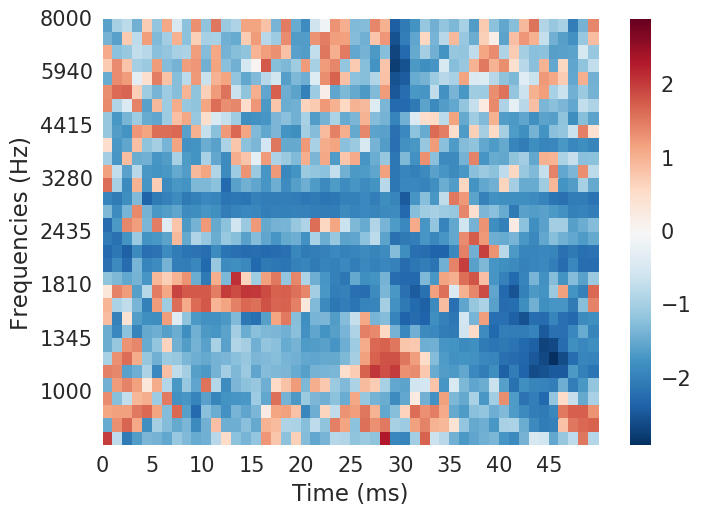
\includegraphics[scale=0.3,valign=t]{images-data/ild}
	\caption{ILD feature}
	\label{fig:methods:ild}
\end{subfigure}~
\begin{subfigure}[t]{0.3\textwidth}
	\hspace*{-0.5cm}
	\centering
	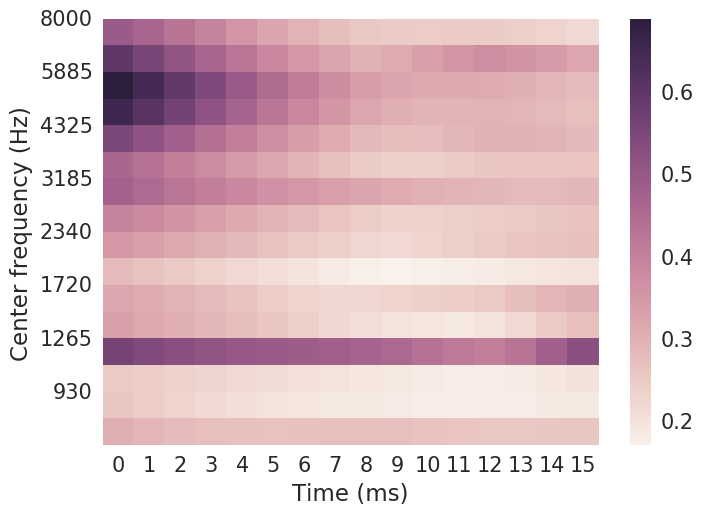
\includegraphics[scale=0.3,valign=t]{images-data/ams}
	\caption{Left-channel first AMS}
	\label{fig:methods:ams}
\end{subfigure}~
\begin{subfigure}[t]{0.3\textwidth}
	\centering
	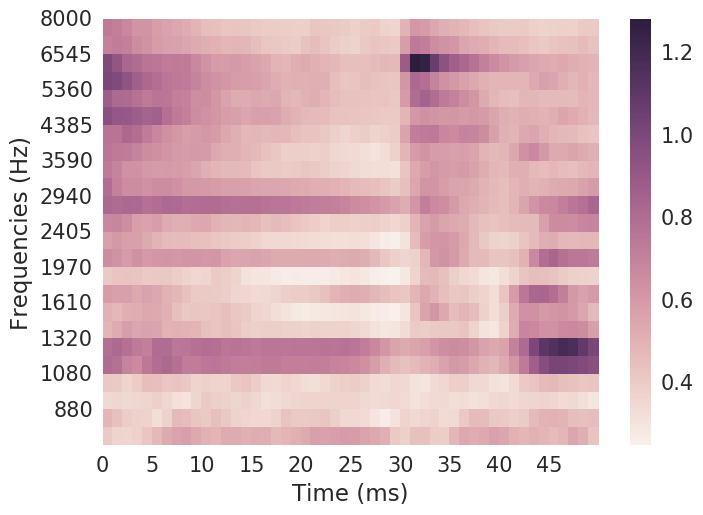
\includegraphics[scale=0.3,valign=t]{images-data/rmp}
	\caption{Left-channel ratemap}
	\label{fig:methods:rmp}
\end{subfigure}
\caption{Features representation for a "phone" recording (ILD, AMS and ratemap)}
\end{figure}

\subsection{Balancing}
\label{sec:methods:balancing}

All types of classes are originally strongly imbalanced for both types of sounds. That means some classes are outnumbered by other classes. That could possibly lead to a bias towards the majority classes, treating minority classes as outliers or even not considering rare events at all. This phenomenon applies to identifications classes (class count in figure~\ref{fig:methods:class_count_clean}), localization classes (azimuths count in figure~\ref{fig:methods:class_count_azimuths}) and number of sources (counted for one specific class in figure~\ref{fig:methods:class_count_sources}).

Balancing is performed by counting each class and fixing a target as the exact class count we want to reach for each class after balancing. Minority classes are artificially oversampled by repeating elements from the class; majority classes are subsampled.
\begin{figure}[htb]
\begin{subfigure}[t]{0.5\textwidth}
	\centering
	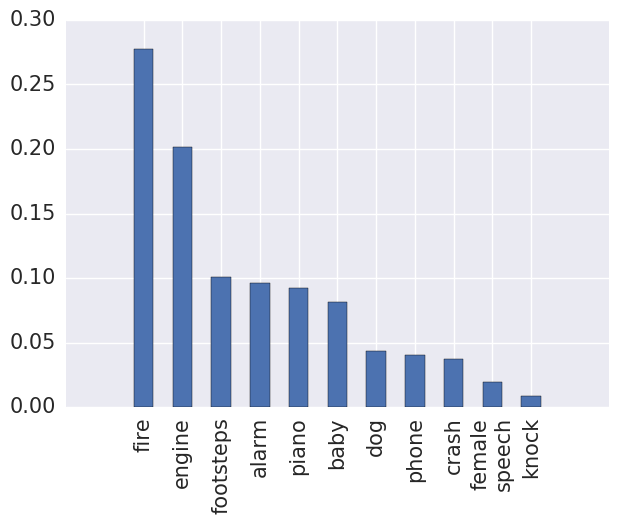
\includegraphics[scale=0.4,valign=t]{images-data/class_count_clean}
	\caption{Identification classes for clean sounds}
	\label{fig:methods:class_count_clean}
\end{subfigure}%
\begin{subfigure}[t]{0.5\textwidth}
	\centering
	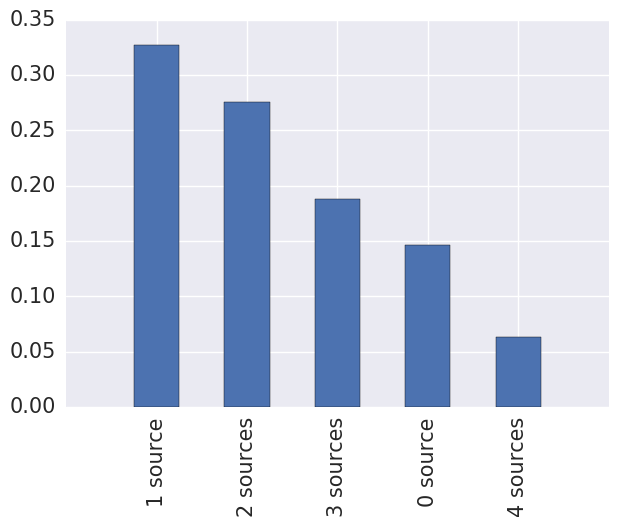
\includegraphics[scale=0.4,valign=t]{images-data/class_count_sources}
	\caption{Co-occurent sources for mixed sounds}
	\label{fig:methods:class_count_sources}
\end{subfigure}
\begin{subfigure}[t]{\textwidth}
	\centering
	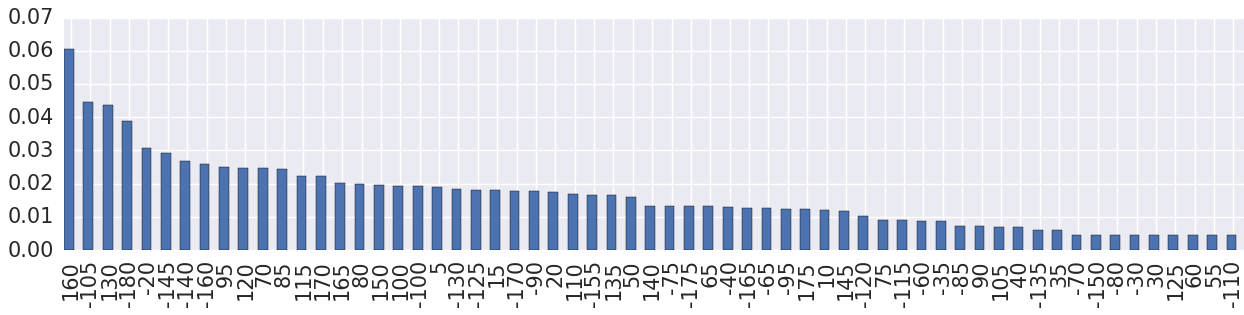
\includegraphics[scale=0.45]{images-data/class_count_azimuths}
	\caption{Distribution of azimuths for the class "alarm" of the mixed sounds (sorted according to frequencies of localization classes)}
	\label{fig:methods:class_count_azimuths}
\end{subfigure}
\label{fig:methods:balancing}
\caption{Percentage ratio of several classes for clean and mixed sounds (while some classes stand out, others are outnumbered)}
\end{figure}

Although balancing was performed for identification classes, it has not been solved on mixed sounds in the azimuth plane. Balancing one class type (\textit{e.g.} azimuths) would indeed tend to imbalance another one (\textit{e.g.} number of sources). That is why azimuth imbalance was not tackled for mixed sounds.

\subsection{Train-test split}

After balancing, clean sounds count \num[group-separator={,}]{9000000} data points and mixed sounds count \num[group-separator={,}]{17227800} data points. They are first randomly shuffled in order to not bias the gradient with entire batches of highly correlated examples, which could lead to a poor convergence (see the gradient descent algorithm in section~\ref{sec:introduction:deep_learning}). Data points are then split into training and testing sets in the proportion 67\%-33\%.

Training and testing datasets are saved under separate HDF5 files (*.h5). We chose HDF5 format over LMDB for its simplicity in read/write actions and its portability in Python through the \verb+h5py+ library.


%%%%%%%%%%%%%%%%%%%%%%%%%%%%%%%%%%%%%%%%%%%%%%%%%%%%%%%%%
\section{Evaluation metrics}
\label{sec:methods:metrics}

Machine learning model evaluation requires to work with appropriate evaluation metrics. We here present the metrics that we used for picking the best models.

\subsection{Learning curve}

As described in section~\ref{sec:introduction:deep_learning:cnn}, train and test losses (also called cost errors) are direct outputs of a neural network, so they do not require extra calculations. They are evaluated between the expected ground truths and the obtained labels either on the train set or on the test set with the chosen loss. Plotting the train and test losses as a function of the number of learning iterations is called visualizing the learning curve.

The train loss characterizes the network's learning progression. A flat learning error represents a slow-learning network. When the train loss reaches a plateau, one can say the network is no longer learning. The test loss shows the network's generalization capacity on unseen data.

The test-train difference between the train loss and the test loss characterizes the bias-variance trade-off \parencite{geman1992neural}. A high bias corresponds to a high training error and a small test-train difference, whereas a high variance is characterized  by a huge gap between the test and the train losses (\textit{i.e.} a big test-train difference). The test-train difference can be qualitatively estimated on the learning curve, or quantitatively expressed as a relative difference:
\begin{equation}
\text{Test-train difference} = \min_{\mathbf{w}}\frac{|L_{\text{train}}(\mathbf{w}) - L_{\text{test}}(\mathbf{w})|}{\max\left(L_{\text{train}}(\mathbf{w}), L_{\text{test}}(\mathbf{w})\right)}
\end{equation}

\subsection{Confusion matrix}

A confusion matrix allows to visualize the performance of an algorithm by counting the actual labels \textit{versus} the predicted labels for each given class, as presented in figure \ref{fig:introduction:confusion}.
\begin{figure}[htb] \centering
\begin{tabular}{c|c|ccccccc|}
\multicolumn{2}{c}{} & \multicolumn{7}{c}{Predicted class} \\
\cline{3-5}\cdashline{5-6}\cline{7-9}
\multicolumn{2}{c|}{} & \verb+ Baby + & \verb+ Dog  + & & \ldots & & \verb+ Fire + & \verb+Scream+ \\
\cline{2-5}\cdashline{5-6}\cline{7-9}
\parbox[c]{2mm}{\multirow{7}{*}{\rotatebox[origin=c]{90}{Actual class}}} & \verb+Baby+ & \TN298 & 2 & \multicolumn{3}{c}{} & \FP3 & 6 \\
& \verb+Dog+ & 10 & \TN233 & \multicolumn{3}{c}{} & \FP1 & 61 \\
& & \multicolumn{2}{c}{} & \multicolumn{1}{c}{\TN$\ddots$} & \multicolumn{2}{c}{} & \multicolumn{1}{c}{\FP} & \multicolumn{1}{c|}{} \\
\multicolumn{1}{c:}{} & \multicolumn{1}{c:}{\vdots} & \multicolumn{3}{c}{} & \TN$\ddots$ & \multicolumn{1}{c}{} & \multicolumn{1}{c}{\FP} & \multicolumn{1}{c:}{} \\
& & \multicolumn{4}{c}{} & \multicolumn{1}{c}{\TN$\ddots$} & \multicolumn{1}{c}{\FP} & \multicolumn{1}{c|}{} \\
& \verb+Fire+ & \FN1 & \FN2 & \multicolumn{3}{c}{\FN} & \TP293 & \FN4 \\
& \verb+Scream+ & 5 & 12 & \multicolumn{3}{c}{} & \FP1 & \TN261 \\
\cline{2-5}\cdashline{5-6}\cline{7-9}
\end{tabular}\\
\begin{tabular}{ccccc}
\verb+ + & & & & \\
\TP & True positives ($TP$) & \verb+  + & \FP\verb+ + & False positives ($FP$) \\
\TN & True negatives ($TN$) & & \FN & False negatives ($FN$) \\
\end{tabular}
\caption{Example of confusion matrix with $TP$, $TN$, $FP$ and $FN$ for the class "Fire"}
\label{fig:introduction:confusion}
\end{figure}
From that, we can define sensitivity (also called recall, or true positive rate), specificity (true negative rate) and precision (positive predictive value), such that:
\begin{equation}
\left\{
\begin{aligned}
\text{Sensitivity} & = \text{Recall} = \frac{TP}{TP + FN} & (\text{true positive rate}) \\
\text{Specificity} & = \frac{TN}{TN + FP} & (\text{true negative rate}) \\
\text{Precision} & = \frac{TP}{TP + FP} & (\text{positive predictive value})
\end{aligned}
\right.
\end{equation}
Sensitivity illustrates the classifier's benefits by counting well-classified cases. Specificity depicts the model's ability to classify other classes relatively to a given class. Sensitivity and specificity are inversely proportional, meaning that as the sensitivity increases, the specificity falls and \textit{vice versa}. The precision of the classifier is the percentage of sounds predicted for a given class who actually belong to this class. Precision and sensitivity are also inversely related. The trade-offs between sensitivity \textit{versus} specificity and precision \textit{versus} sensitivity have specific metrics explored in section \ref{methods:metrics:tradeoff}.

\subsection{Overall and balanced accuracy}

\textbf{Overall accuracy} is defined for classifiers as the portion of correctly predicted labels. Accuracy makes sense when used with balanced datasets and softmax activation layers, in which case accuracy reflects the actual performance of the classifier:
\begin{equation}
\text{Accuracy} = \frac{TP + TN}{TP + FP + TN + FN}
\end{equation}
Accuracy requires a properly balanced dataset (which works fine in the case of clean sounds). Imbalanced domains would indeed be biased by a trivial classifier that would always predict the majority classes and ignore rare events. Accuracy can therefore only be computed when dealing with clean sounds and using a softmax activation layer (see equation~\ref{eq:softmax}) which favors one class over all the others for both identification and localization. In the case of imbalanced datasets and/or multilabel classification, other metrics should be used to assess the classification performance, such as balanced accuracy or precision and recall.

\textbf{Balanced accuracy} relates the portion of correctly predicted labels to the number of actual positives and negatives, as in:
\begin{equation}
\text{Balanced accuracy} = \frac{1}{2} \left( \frac{TP}{TP + FN} + \frac{TN}{TN + FP} \right)
\end{equation}
Balanced accuracy can be viewed as the arithmetic mean of sensitivity and specificity (true positive and negative rates). It can be used with mixed sounds. For those classifiers, other metrics were also used such as the receiver operating characteristic and the precision-recall curves.

\subsection{Trade-off between sensitivity, specificity and precision}
\label{methods:metrics:tradeoff}

For the mixed sounds, the classifier outputs a score for each identification and localization class, then converted to a probability through the sigmoid activation layer. A class is considered as active if the obtained probability goes beyond a given threshold. This threshold is arbitrarily $0.5$ by default, but can be changed in order to improve the classifier's performance. Finding the most appropriate threshold can be achieved by plotting the two following curves that aim at finding trade-offs between sensitivity, specificity and precision.

\textbf{Receiver operating characteristic (ROC).} For each class, the ROC curve is defined by the FP rate and the sensitivity as $x$ and $y$-axis for each probability threshold used by the classifier. ROC depicts the trade-off between false positive ($= 1 - \text{specificity}$, i.e. the costs) and true positive ($= \text{sensitivity}$, i.e. the benefits) rates.

\textbf{Precision-recall (PR).} For each class, the PR curve represents the precision and the recall (also called sensitivity) as $x$ and $y$-axis for several probability thresholds. PR thus depicts the trade-off between the classifier's precision and sensitivity.

For both curves, the area under the curve (AUC) is considered an appropriate metrics of the corresponding trade-off. The AUC is calculated by using an average of a number of trapezoidal approximations on several chosen thresholds.

\citeauthor{davis2006relationship} \parencite{davis2006relationship} argue that when a problem suffers from class imbalance, using the PR AUC as evaluation metrics is better than the ROC AUC, so the PR AUC should be favored in case of ambiguity. Both were computed for mixed sounds.


%%%%%%%%%%%%%%%%%%%%%%%%%%%%%%%%%%%%%%%%%%%%%%%%%%%%%%%%%
\section{Architecture selection}

The architecture selection aims at picking the best models in terms of accuracy. This requires to select the:%
\begin{itemize}
\itemsep-1em
\item features that will be used (feature selection): ratemaps, AMS or ILD features, or any combination of them,
\item network's depth for the convolutional layers and the inner products,
\item hyperparameter for the layers (e.g. number of filters, size of filters and stride for convolutional layers) and the solver (e.g. learning rate and momentum used by the stochastic gradient descent).
\end{itemize}

\subsection{Convolutional neural networks}

As illustrated on the example of the figure \ref{fig:introduction:convnet}, we focus on the class of neural networks of the following form:

\begin{figure}[htb]
\hspace*{-1cm}
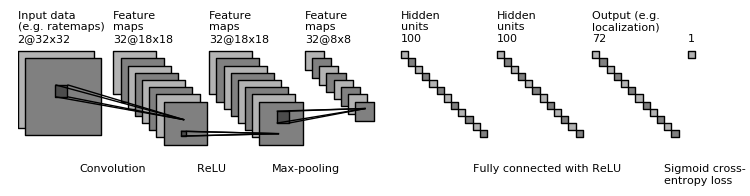
\includegraphics[scale=0.85]{images-data/convnet_fig}
\caption{Simple CNN architecture with one convolutional stage and two inner products}
\label{fig:introduction:convnet}
\end{figure}

\textbf{Convolutional stages.} We stack from one to three convolutional stages with their filter layers (hyperparameters: number of filters, size of filters, stride), non-linear layers (no hyperparameter for ReLUs) and dimension reduction layers using max pooling (hyperparameter: stride).

\textbf{Fully connected layers.} We stack from one to two inner products (hyperparameter: number of nodes) including dropout in the training phase.

\textbf{Activation layers.} They are sigmoid layers for the mixed sounds and softmax layers for the clean sounds. The softmax function allows to make a class stand out through the use of exponential coefficients,---thus achieving multiclass unilabel classification. The sigmoid function on the contrary only converts values from the last fully connected layer to related probabilities in the range $[0,1]$. In mathematical terms, we have for $j = 1,\dotsc,K$ (indices of the last inner product):
\begin{equation}
\left\{
\begin{aligned}
\text{Sigmoid: } & \sigma (\mathbf{z})_j = \frac{1}{1 + e^{-\mathbf{z}_j}} \\
\text{Softmax: } & \sigma (\mathbf{z})_j = \frac{e^{\mathbf{z}_j}}{\sum_{k=1}^K e^{\mathbf{z}_k}}
\label{eq:softmax}
\end{aligned}
\right.
\end{equation}

\subsection{Methods for hyperparameter optimization}
\label{methods:architecture:random}

\textbf{Manual optimization.} Going from coarse to fine on the hyperparameter ranges, we manually update the hyperparameters and check for the obtained accuracy. In addition to being relatively slow, this search is not optimal and only gives a sense of what may happen underneath. It requires an expert experience, as well as the knowledge of unwritten rules of thumbs.

\textbf{Grid search} consists of an exhaustive search on the whole hyperparameter space, each combination of hyperparameters being mapped to their respective accuracy. While this technique is particularly relevant for most machine learning algorithms, it is not well suited to neural networks where hyperparameters are numerous and lie in a highly dimensional space.

\textbf{Bayesian optimization} aims at efficiently navigating within the hyperparameter space. Spearmint \parencite{snoek2012practical} is an open-source Python library that can be used for that purpose. The Bayesian strategy treats the evaluation metrics as a random function with a prior over it (pre-knowledge). As models are trained, the prior is updated to form the posterior distribution which is in turn used to find the most appropriate hyperparameters that determine the next model to train.

\textbf{Random search} consists of a random search on the hyperparameter space. It is proved more efficient in time and computing power than a regular exhaustive grid search, because not all hyperparameters are equally important to tune \parencite{bergstra2012random}. We implemented a random search for Caffe and used it for models with clean and mixed sounds. For each architecture to investigate, the hyperparameters are randomly initialized, the network is trained for a given number of iterations and its performance is assessed through well-chosen evaluation metrics. When selecting models with random search, we proceed from coarse to fine in terms of depth and complexity of the tested architectures. In this manner, we can reuse the weights at each random iteration and need less learning iterations before convergence. % INCLUDE: related work
\chapter{Results}
\label{sec:results}


%%%%%%%%%%%%%%%%%%%%%%%%%%%%%%%%%%%%%%%%%%%%%%%%%%%%
\section{Architecture selection on clean sounds}
\label{sec:results:clean}

For the architecture selection, we use random search as described in section~\ref{methods:architecture:random}. Several architectures can thus be tested and their relative performances compared. The metrics we used are the test accuracy (in mean and maximum), the test loss (in mean) and the test-train difference (in relative difference). For the architecture selection, we favored identification over localization as localization is proved easier to learn as seen in section~\ref{sec:results:multi}.

The tested architectures are presented on table~\ref{fig:results:clean_table} and compared on figures~\ref{fig:results:max_test_accuracy}~to~\ref{fig:results:test_train_diff}.

\renewcommand{\arraystretch}{1.5}
\begin{table}[htb]
\begin{tabular}{|p{.25\textwidth}|p{.75\textwidth}|}
\hline
\verb+rmp_1conv_2ip+ & Using only ratemaps, one convolutional stage followed by two inner products \\
\hline
\verb+rmp_2conv_1ip+ & Using only ratemaps, two convolutional stages followed by one inner product \\
\hline
\verb+rmp_2conv_2ip+ & Using only ratemaps, two convolutional stages followed by two inner products \\
\hline
\verb+rmp_3conv_1ip+ & Using only ratemaps, three convolutional stages followed by one inner product \\
\hline
\verb+ams_1conv_2ip+ & Using only AMS, one convolutional stage followed by two inner products \\
\hline
\verb+amsrmp_2conv_2ip+ & Using all available features (AMS and ratemaps), two convolutional stages followed by two inner products \\
\hline
\verb+amsrmp_2conv_2ip+ & Using AMS and ratemaps, two convolutional stages followed by two inner products \\
\hline
\verb+amsrmp_2dconv_1ip+ & Using AMS and ratemaps, two parallel convolutional stages for both features followed by a concatenation stage and one single inner product; the models learn different weights for the two convolutions; the parameters of the convolution however are the same, so that they produce outputs of the same size that can be concatenated \\
\hline
\end{tabular}
\\
\caption{Tested architectures for clean sounds}
\label{fig:results:clean_table}
\end{table}

\begin{figure}[htb]
\label{fig:results:clean}
\begin{subfigure}[t]{0.5\textwidth}
	\centering
	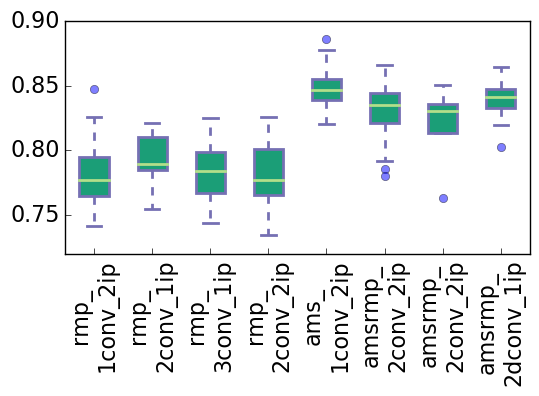
\includegraphics[scale=0.5]{images-architecture-clean/max_test_accuracy}
    \caption{Test accuracy in maximum}
	\label{fig:results:max_test_accuracy}
\end{subfigure}%
\begin{subfigure}[t]{0.5\textwidth}
	\centering
	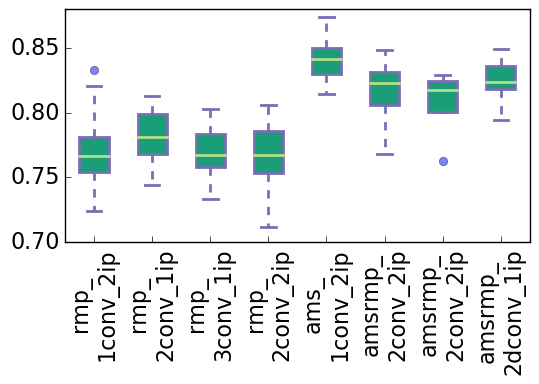
\includegraphics[scale=0.5]{images-architecture-clean/mean_test_accuracy}
    \caption{Test accuracy in mean}
	\label{fig:results:mean_test_accuracy}
\end{subfigure}
\begin{subfigure}[t]{0.5\textwidth}
	\centering
	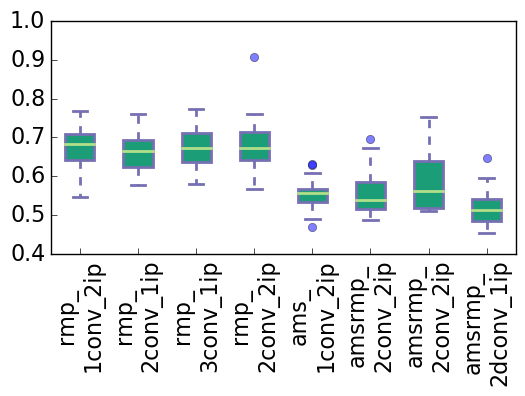
\includegraphics[scale=0.5]{images-architecture-clean/mean_test_loss}
    \caption{Test loss in mean on final plateau}
	\label{fig:results:mean_test_loss}
\end{subfigure}%
\begin{subfigure}[t]{0.5\textwidth}
	\centering
	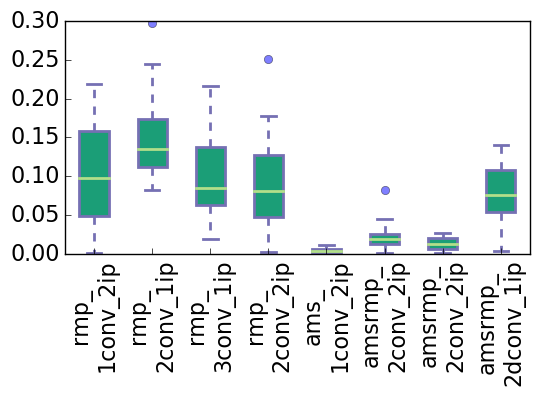
\includegraphics[scale=0.5]{images-architecture-clean/test_train_diff}
    \caption{Test-train difference}
	\label{fig:results:test_train_diff}
\end{subfigure}
\caption{Architecture selection results for clean sounds using several features and depths}
\end{figure}
The architecture using only AMS with one convolutional stage and two inner products (\verb+ams_1conv_2ip+) clearly stands out for all metrics with an accuracy mean of 87.4\% for identification.


%%%%%%%%%%%%%%%%%%%%%%%%%%%%%%%%%%%%%%%%%%%%%%%%%%%%
\section{Multitask learning on clean sounds}
\label{sec:results:multi}

We here intend to compare the learning speed and final performance of different multitask learning techniques, based on the same best model of section~\ref{sec:results:clean}. The tested architectures are presented on table~\ref{fig:results:multitask} and compared on figures~\ref{fig:results:id_test_accuracy} to~\ref{fig:results:loc_train_loss}.

\renewcommand{\arraystretch}{1.5}
\begin{table}[htb]
\begin{tabular}{|p{.15\textwidth}|p{.85\textwidth}|}
\hline
\verb+Id, loc+ & Sequential multitask learning starting with identification before learning both tasks \\
\hline
\verb+Loc, id+ & Sequential multitask learning starting with localization before learning both tasks \\
\hline
\verb+Joint+ & Joint multitask learning with all branches in common; only the output layers are task-specific; both losses have the same weight and are simultaneously optimized \\
\hline
\verb+Joint, sep+ & Joint multitask learning with the last layers optimized simultaneously, but separately (i.e. with different learnt weights) \\
\hline
\end{tabular}
\\
\caption{Tested architectures for multitask learning}
\label{fig:results:multitask}
\end{table}

All experiments were launched with the same training and testing parameters, so they can be properly compared. We took a moving average of the training loss on the last $30$ iterations, in order to smooth the learning curve and extract the global pattern.

\begin{figure}[htb]
\begin{subfigure}[t]{0.5\textwidth}
	\centering
	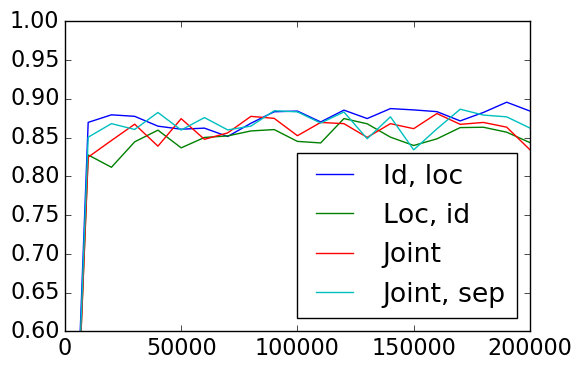
\includegraphics[scale=0.45]{images-architecture-compare/id_test_accuracy}
    \caption{Identification test accuracy}
	\label{fig:results:id_test_accuracy}
\end{subfigure}%
\begin{subfigure}[t]{0.5\textwidth}
	\centering
	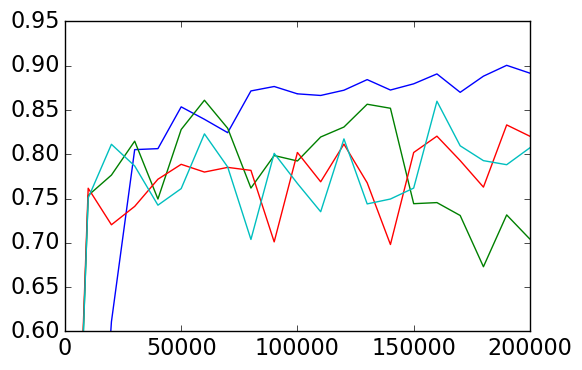
\includegraphics[scale=0.45]{images-architecture-compare/loc_test_accuracy}
    \caption{Localization test accuracy}
	\label{fig:results:loc_test_accuracy}
\end{subfigure}
\begin{subfigure}[t]{0.5\textwidth}
	\centering
	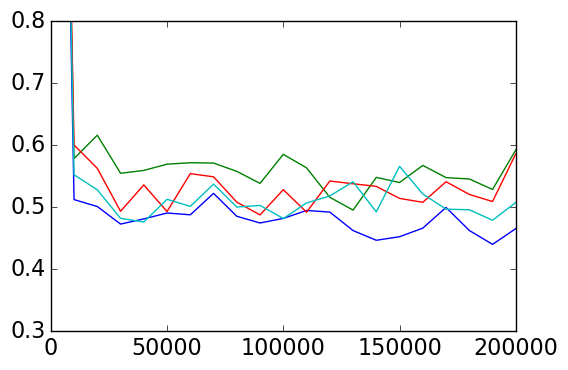
\includegraphics[scale=0.45]{images-architecture-compare/id_test_loss}
    \caption{Identification test loss}
	\label{fig:results:id_test_loss}
\end{subfigure}%
\begin{subfigure}[t]{0.5\textwidth}
	\centering
	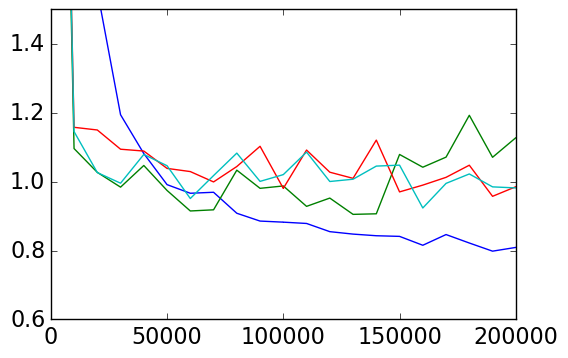
\includegraphics[scale=0.45]{images-architecture-compare/loc_test_loss}
    \caption{Localization test loss}
	\label{fig:results:loc_test_loss}
\end{subfigure}
\begin{subfigure}[t]{0.5\textwidth}
	\centering
	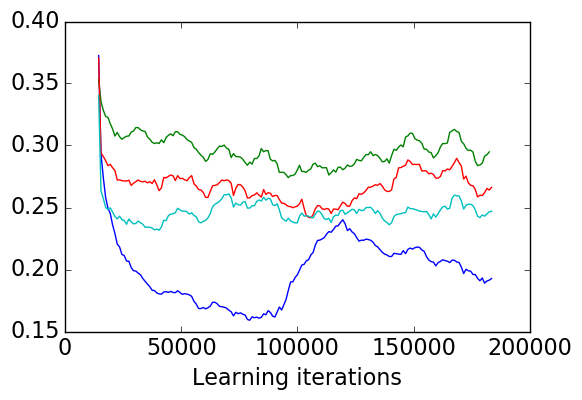
\includegraphics[scale=0.45]{images-architecture-compare/id_train_loss}
    \caption{Averaged identification train loss}
	\label{fig:results:id_train_loss}
\end{subfigure}%
\begin{subfigure}[t]{0.45\textwidth}
	\centering
    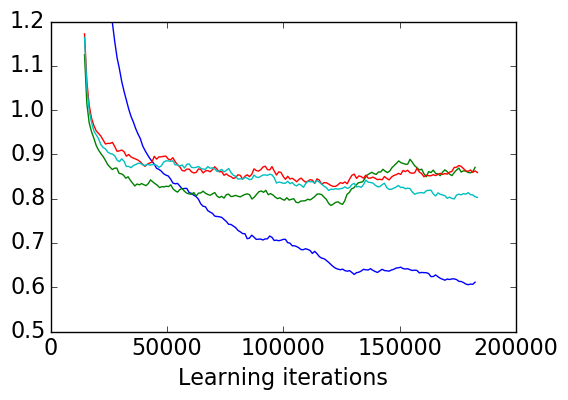
\includegraphics[scale=0.45]{images-architecture-compare/loc_train_loss}
    \caption{Averaged localization train loss}
    \label{fig:results:loc_train_loss}
\end{subfigure}
\caption{Learning curves with different multitask learning techniques for both tasks (identification on the left, localization on the right)}
\end{figure}

First of all, the convergence speeds to the desired plateau accuracies in \ref{fig:results:id_test_accuracy} and \ref{fig:results:loc_test_accuracy} confirm that identification is easier to learn for the network than localization.
We also notice that fine-tuning for multitask learning beginning with identification (i.e. the "easiest" task in terms of learning) seems more efficient, in that its test accuracy (the blue line in \ref{fig:results:id_test_accuracy} and \ref{fig:results:loc_test_accuracy}) converges much faster to the optimal accuracy for the desired tasks. Using fine-tuning would also allow to prioritize one task over another, in particularly by decreasing the learning rate or increasing the momentum after having trained one task. The second task to be trained will take some time to adjust as seen in \ref{fig:results:id_train_loss} and \ref{fig:results:loc_train_loss}. We finally achieve best plateau accuracies (best mean on the last 20\% plateau of the accuracy function) of 88.8\% for identification and 88.7\% for localization.

Secondly, for both identification and localization, there is a difference in the learning speed between the joint learning and the joint learning on separate branches as seen on \ref{fig:results:id_train_loss} and \ref{fig:results:loc_train_loss}. In mean, the training loss using full joint learning is 9\% higher than the training loss using separate branches for identification, and 5\% higher for localization. This means that the last layers of a CNN would construct features that are less transferable than early layers. As \citeauthor{yosinski2014transferable} \parencite{yosinski2014transferable} also argue, this supports the fact that first-layer features are general while last-layer features are more specific to the trained task. However, in our case, further experiments should be led with various architectures, in order to draw more general conclusions. In particularly, this phenomenon should be proved to be independent from the weight and bias initializations, which are currently set to random in all our experiments, as customary in deep learning. In that matter, averaging results on several learning and test phases can lead to more robust results.


%%%%%%%%%%%%%%%%%%%%%%%%%%%%%%%%%%%%%%%%%%%%%%%%%%%%
\section{Architecture selection on mixed sounds}
\label{sec:results:mixed}

As for mixed sounds, we also use random search as described in section~\ref{methods:architecture:random}. We did not rely on the architectures we found for clean sounds, as the data, the features and the complexity of the problem are all very different. The several models are compared by their test losses (in mean) and test-train loss differences (in relative difference), as other metrics require more expensive computations which are not compatible with random search.

The tested architectures are presented on table~\ref{fig:results:mixed_table} and compared on figures~\ref{fig:results:mean_test_loss_mixed} ~and~\ref{fig:results:test_train_diff_mixed}.
\renewcommand{\arraystretch}{1.5}
\begin{table}[htb]
\begin{tabular}{|p{.25\textwidth}|p{.75\textwidth}|}
\hline
\verb+ild_1conv2ip+ & Using ILD features only, one convolutional stage followed by two inner products \tabularnewline
\hline
\verb+all_1conv2ip_10x10+ & Using all available features (AMS, ILD and ratemaps), one convolutional stage followed by two inner products; the first convolutions are adjusted so that it produces outputs of the same size $10\times10$ for each feature, which can then be concatenated and fed into the inner products \tabularnewline
\hline
\verb+all_1conv2ip_12x16+ & With all features, one convolutional stage followed by two inner products; the first convolution outputs features of size $12\times16$ \tabularnewline
\hline
\verb+all_1conv2ip_16x16+ & With all features, one convolutional stage followed by two inner products; the first convolutions output features of size $16\times16$ \tabularnewline
\hline
\verb+all_2conv2ip_16x16+ & With all features, two convolutional stages followed by two inner products; the first convolution is as described above \tabularnewline
\hline
\verb+all_3conv2ip_16x16+ & With all features, three convolutional stages followed by two inner products; the first convolution is as described above \\
\hline
\end{tabular}
\\
\caption{Tested architectures for mixed sounds}
\label{fig:results:mixed_table}
\end{table}
\begin{figure}[htb]
\begin{subfigure}[t]{0.5\textwidth}
	\centering
	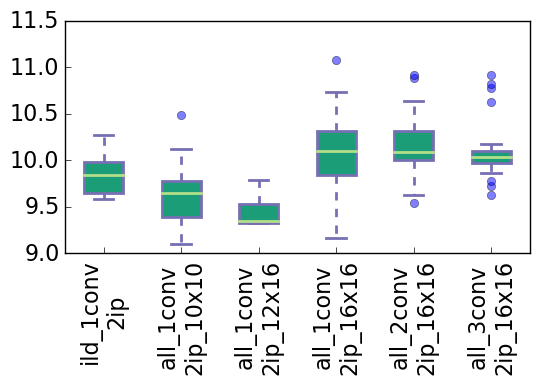
\includegraphics[scale=0.5]{images-architecture-mixed/mean_test_loss}
    \caption{Test loss in mean on final plateau}
	\label{fig:results:mean_test_loss_mixed}
\end{subfigure}%
\begin{subfigure}[t]{0.5\textwidth}
	\centering
	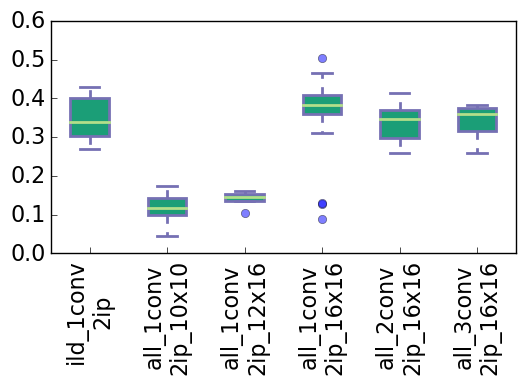
\includegraphics[scale=0.5]{images-architecture-mixed/test_train_diff}
    \caption{Test-train difference}
	\label{fig:results:test_train_diff_mixed}
\end{subfigure}
\caption{Architecture selection results for mixed sounds using several features and depths}
\end{figure}
We first tested each feature taken individually (results using only ratemaps and only AMS are relatively too poor to appear on the figures), then all features with architectures of increasing depths. As features have different sizes, the first convolutions are arranged to output features of same sizes that can then be processed in the rest of the network. For this purpose, we exploit the relationship in a convolution between the output size $W_{\text{ouput}}$, the input size $W_{\text{input}}$, the size $F$ of the convolution filter, the stride $S$ and the padding $P$ with which they are applied:
\begin{equation}
W_{\text{output}} = \frac{W_{\text{input}} - F + 2P}{S + 1}
\end{equation}

In this case, the test-train difference makes less sense because random search does not allow to train long enough to make training and test losses comparable. We retain three architectures with the three best test losses (\verb+all_1conv2ip_16x16+, \verb+all_2conv2ip_16x16+ and \verb+all_3conv2ip_16x16+).


%%%%%%%%%%%%%%%%%%%%%%%%%%%%%%%%%%%%%%%%%%%%%%%%%%%%
\section{Multitask learning performances on mixed sounds}
\label{sec:results:perf}

The best performing model from section~\ref{sec:results:mixed} is picked to be assessed using the specific metrics of section~\ref{sec:methods:metrics} (Evaluation metrics).

The best-identified classes by increasing order of ROC AUC are as shown on figure~3.4:
dog (0.778 ROC AUC),
female and male screams (0.763),
female speech (0.733),
knock (0.731),
male speech (0.723),
baby (0.709),
engine (0.706),
piano (0.702),
alarm (0.67),
fire (0.662),
phone (0.638),
footsteps (0.635) and
crash (0.609).

\begin{figure}
\hspace*{-2cm}
\centering
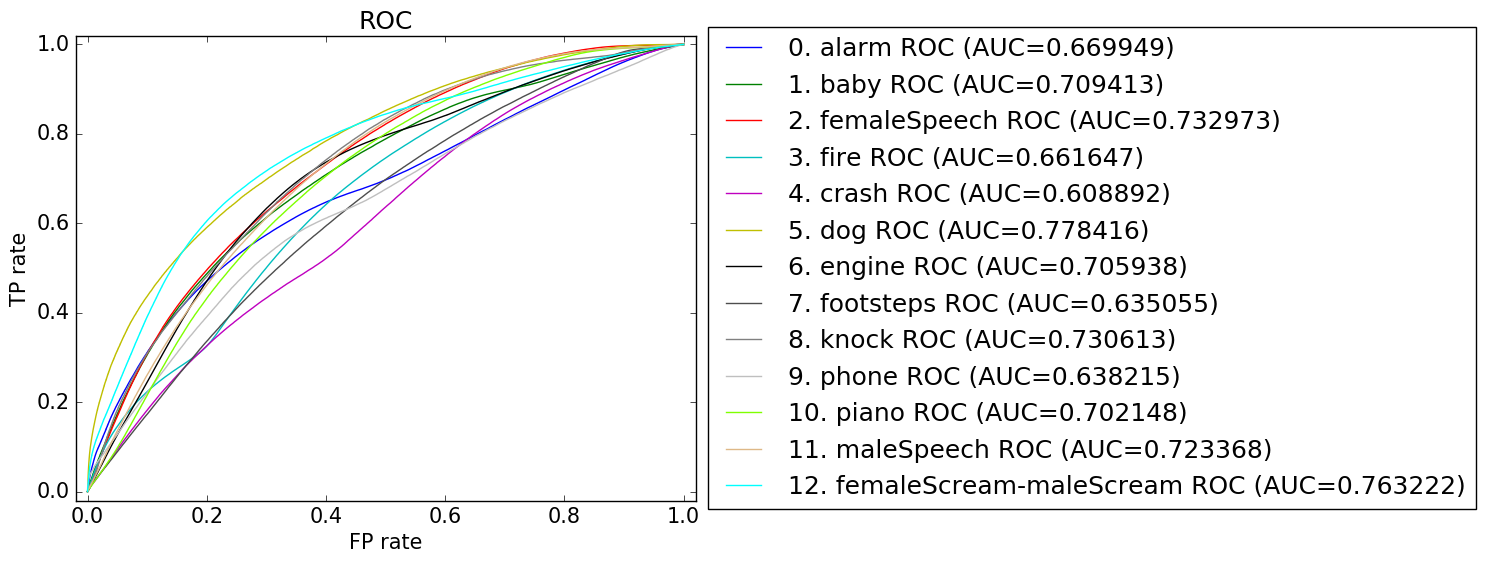
\includegraphics[scale=0.45]{images-architecture-mixed/id_roc}
\label{fig:results:id_roc}
\caption{Area under the curve of the receiving operating curve (AUC ROC) for identification classes}
\end{figure}

The maximal balanced accuracy calculated at the best classifier threshold also gives similar results as shown on figure~3.5:
female and male screams (70.95\% balanced accuracy),
dog (69.99\%),
knock (67.13\%),
engine (67.1\%),
male speech (66.71\%),
female speech (66.59\%),
baby (65.7\%),
piano (65.36\%),
alarm (63.88\%),
fire (62.4\%),
phone (61.5\%),
footsteps (59.93\%) and
crash (57.56\%). With both metrics, screams are the best-identified class.

\begin{figure}
	\hspace*{-4cm}
	\centering
	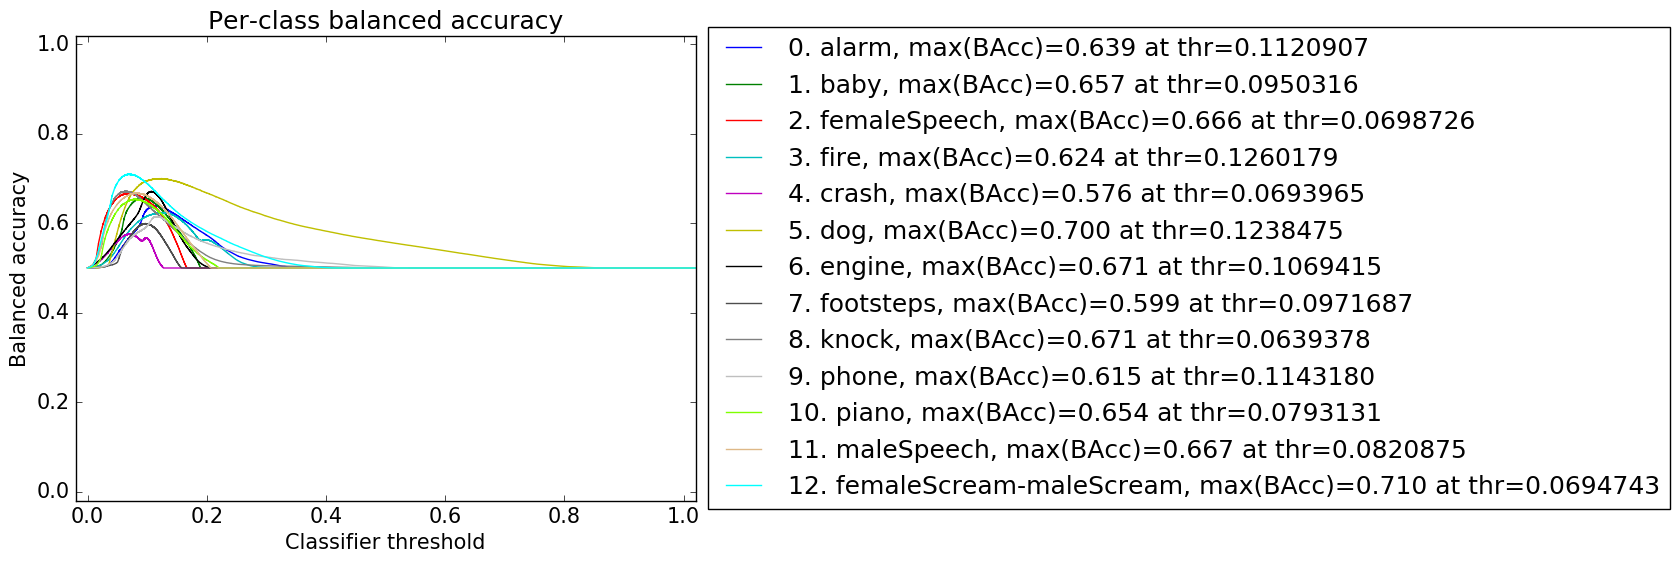
\includegraphics[scale=0.45]{images-architecture-mixed/id_max_bacc}
	\label{fig:results:id_max_bacc}
\caption{Identification classes balanced accuracy calculated for each classifier threshold}
\end{figure}

As for localization, balanced accuracy clearly indicates that the agent only achieves a near-chance performance, averaging at 53.15\% balanced accuracy, as shown in figure~3.6a. However the best-localized classes are:
-160.0$^\circ$ (60.05\% balanced accuracy),
-150.0$^\circ$ (59.23\%),
-100.0$^\circ$ (57.93\%),
-65.0$^\circ$ (56.66\%),
-90.0$^\circ$ (56.29\%),
-105.0$^\circ$ (55.63\%),
-180.0$^\circ$ (55.39\%),
-170.0$^\circ$ (55.23\%),
-140.0$^\circ$ (54.9\%) and
-130.0$^\circ$ (54.07\%).
However, figure~3.6b implies there is a correlation between the frequency of apparition of the azimuth in the training set and the obtained balanced accuracy for the corresponding azimuth. The dataset imbalance in terms of localization classes (as seen on figure~2.3c of section~\ref{sec:methods:balancing}) thus seems to penalize under-representated classes. Sufficient amounts of data is indeed essential for CNN to perform well and that can explain the gap between some localization classes. \\

\begin{figure}[htb]
\begin{subfigure}[t]{0.5\textwidth}
\hspace*{-1cm}
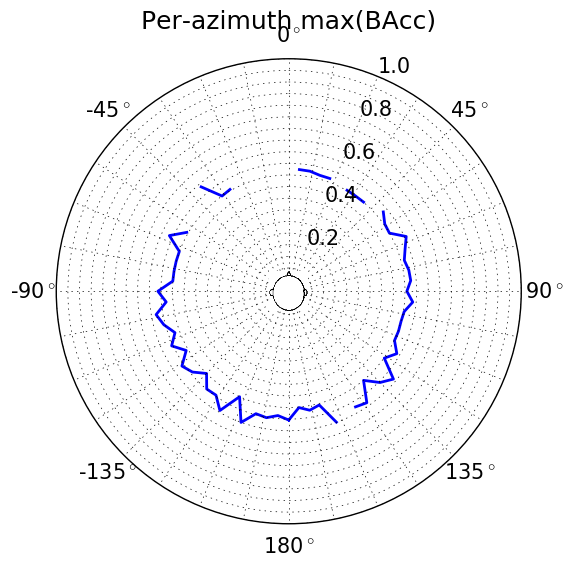
\includegraphics[scale=0.45]{images-architecture-mixed/loc_max_bacc}
\vspace*{.5cm}
\label{fig:results:loc_max_bacc}
\caption{Maximal balanced accuracy at best \\ classifier threshold for localization \\ classes}
\end{subfigure}
\begin{subfigure}[t]{0.5\textwidth}
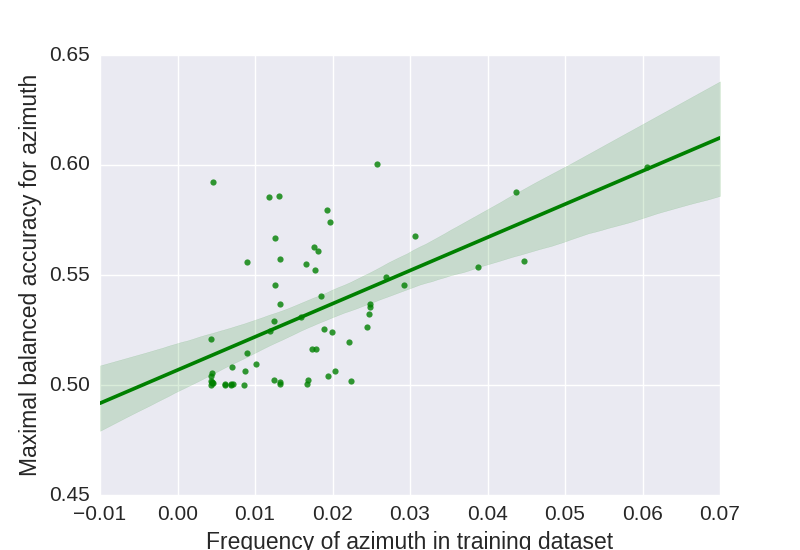
\includegraphics[scale=0.45]{images-data/frequency_accuracy}
\label{fig:results:frequency_accuracy}
\caption{Correlation between the dataset imbalance and the obtained balanced accuracy for each azimuth (regression line and 95\% confidence interval)}
\end{subfigure}
\caption{Results for localization of mixed sounds: balanced accuracy for each azimuth and correlation with localization class percentage ratio}
\end{figure}	% INCLUDE: system
\chapter{Conclusion}
\label{sec:conclusion}

In the present thesis, we were to apply canonical methods of machine and deep learning (such as feature engineering, metrics selection and hyperparameter optimization) to simultaneously localize and classify environmental sounds. After extracting adapted features from regular audio recordings, proper training and testing datasets were prepared for both clean and mixed sounds. Specific evaluation metrics were picked to tackle a multiclass multilabel classification problem. The machine-hearing agent is based on convolutional neural networks whose architectures were iteratively determined through random search.

The real-scenario's complexity (with a variable number of sounds from more identification classes at different azimuths), as well as the presence of reverberation and the strong dataset imbalance make the learning process much more difficult than in the case of clean sounds where we achieve very good levels of accuracy for both identification (88.8\% accuracy) and localization (88.7\% accuracy). For mixed sounds, localization turned out a much harder task (53.2\% balanced accuracy on average) while much better results were achieved for identification (65.0\% balanced accuracy on average).

Further investigations can be done in the future, especially to achieve better results when dealing with mixed sounds. One possibility would be to use deeper networks or longer training time with lowered learning rates. The fact that some localization classes clearly stand out in terms of balanced accuracy indicate better results can also be achieved for other azimuths. Dataset imbalance for mixed sounds was proven to play a role in the poorer results for the localization of some azimuths, so gathering more data for the outnumbered localization classes could help reach better results. Another possibility for achieving better results is to make use of more regularization. An idea for regularization is to convolve in the channel's direction for AMS and ILD features before convolving on each spectrogram.
One could also explore feature transferability by expanding the experiments from section~\ref{sec:results:multi}. In particularly, testing several architectures with multiple random initializations could lead to broader conclusions on layers roles in function of their depths. % INCLUDE: concepts
\cleardoublepage

% --------------------------
% Back matter
% --------------------------
{%
\setstretch{1.1}
\renewcommand{\bibfont}{\normalfont\small}
\setlength{\biblabelsep}{0pt}
\setlength{\bibitemsep}{0.5\baselineskip plus 0.5\baselineskip}
\printbibliography[nottype=online]
%\printbibliography[heading=subbibliography,title={Webseiten},type=online,prefixnumbers={@}] %% REMETTRE CA POUR COMPILER
}
\cleardoublepage

\renewcommand{\listfigurename}{List of Figures and Tables} % List of figures
\listoffigures
\cleardoublepage

%\listoftables
%\cleardoublepage

%% !TEX root = ../thesis-example.tex
%
\pagestyle{empty}
\hfill
\vfill
\pdfbookmark[0]{Colophon}{Colophon}
\section*{Colophon}

This thesis was typeset with \LaTeXe.
It uses the \textit{Clean Thesis} style developed by Ricardo Langner.
The design of the \textit{Clean Thesis} style is inspired by user guide documents from Apple Inc.

Download the \textit{Clean Thesis} style at \url{http://cleanthesis.der-ric.de/}.

%\cleardoublepage

% !TEX root = ../thesis-example.tex
%
%************************************************
% Declaration
%************************************************
\pdfbookmark[0]{Declaration}{Declaration}
\chapter*{Declaration}
\label{sec:declaration}
\thispagestyle{empty}

\textbf{Statutory declaration}. I declare that I have authored this thesis independently, that I have not used other than the declared sources \& resources, and that I have explicitly marked all material which has been quoted either literally or by content from the used sources. 

\textbf{Eidesstattliche Erklärung}. Hierbei erkl\"are ich an Eides statt, dass ich die vorliegende Arbeit selbstst\"andig und ohne
unerlaubte fremde Hilfe angefertigt, andere als die angegebenen Quellen und Hilfsmittel
nicht benutzt und die den benutzten Quellen w\"ortlich oder inhaltlich entnommenen Stellen
als solche kenntlich gemacht habe.

\bigskip

\noindent\textit{\thesisUniversityCity, \thesisDate}

\smallskip

\begin{flushright}
	\begin{minipage}{5cm}
		\rule{\textwidth}{1pt}
		\centering\thesisName
	\end{minipage}
\end{flushright}

%*****************************************
%*****************************************

\clearpage
\newpage
\mbox{}

% **************************************************
% End of Document CONTENT
% **************************************************
\end{document}
